\chapter{Umsetzung der String-Selektion mit Lane Refill}
\label{apx:equals_lane_refill}

\begin{lstlisting}[language=MyC++,
caption=Umsetzung der String-Selektion mit Lane Refill]
// shared memory for the divergence buffers
__shared__ int search_id_divergence_buffer[THREAD_COUNT];
__shared__ int current_divergence_buffer[THREAD_COUNT];

unsigned warpid = (threadIdx.x / 32);	// index of warp in block
unsigned bufferbase = (warpid * 32);    // buffer offset for warp in block
unsigned warplane = (threadIdx.x % 32); // index of lane in warp
unsigned prefixlanes = (0xffffffff >> (32 - warplane)); // previous lanes
int bufferelements = 0;        // number of elements in buffer

while(!flush_pipeline) {
	current = loop_var;
	
	/* execute previous operators in the pipeline */
	
	data_length = char_offset[current+1] - char_offset[current] - 1;
	
	// if string lengths are unequal, discard
	if (active && data_length != search_length)
		active = false;
	
	int numactive = __popc(__ballot_sync(ALL_LANES, active));
	while(bufferelements + numactive > THRESHOLD) {
	
		// refill empty lanes from buffer in case of underutilization
		if (numactive < THRESHOLD) {
			numRefill = min(32 - numactive, bufferelements);
			numRemaining = bufferelements - numRefill;
			
			previous_inactive = __popc(~__ballot_sync(ALL_LANES, active) & prefixlanes);
			
			if (!active && previous_inactive < bufferelements) {
				buf_ix = numRemaining + previous_inactive + bufferbase;
				search_id = search_id_divergence_buffer[buf_ix];
				current = current_divergence_buffer[buf_ix];
				active = true;
			}
			
			bufferelements -= numRefill;
		}
	
		int data_id = search_id + char_offset[current];
		
		// when strings don't match, inactivate the lane
		if (active && data_content[data_id] != search_string[search_id])
			active = false;
		
		search_id++;
		
		if (search_id == search_length) {
		
			/* execute following operators in the pipeline */
		
			active = false;
		}
		
		numactive = __popc(__ballot_sync(ALL_LANES, active));
	}
	
	// flush active lanes to buffer
	if (numactive > 0) {
		previous_active = __popc(__ballot_sync(ALL_LANES, active) & prefixlanes);
		buf_ix = bufferbase + bufferelements + previous_active;
		
		if(active) {
			search_id_divergence_buffer[buf_ix] = character_index;
			current_divergence_buffer[buf_ix] = current;
		}
		
		bufferelements += numactive;
		active = false;
	}
	
	loop_var += step;
}
\end{lstlisting}

\chapter{Laufzeiten für alternative Selektivität des Type-Datensatzes}
\label{apx:parameter64}

\begin{figure}[ht]
	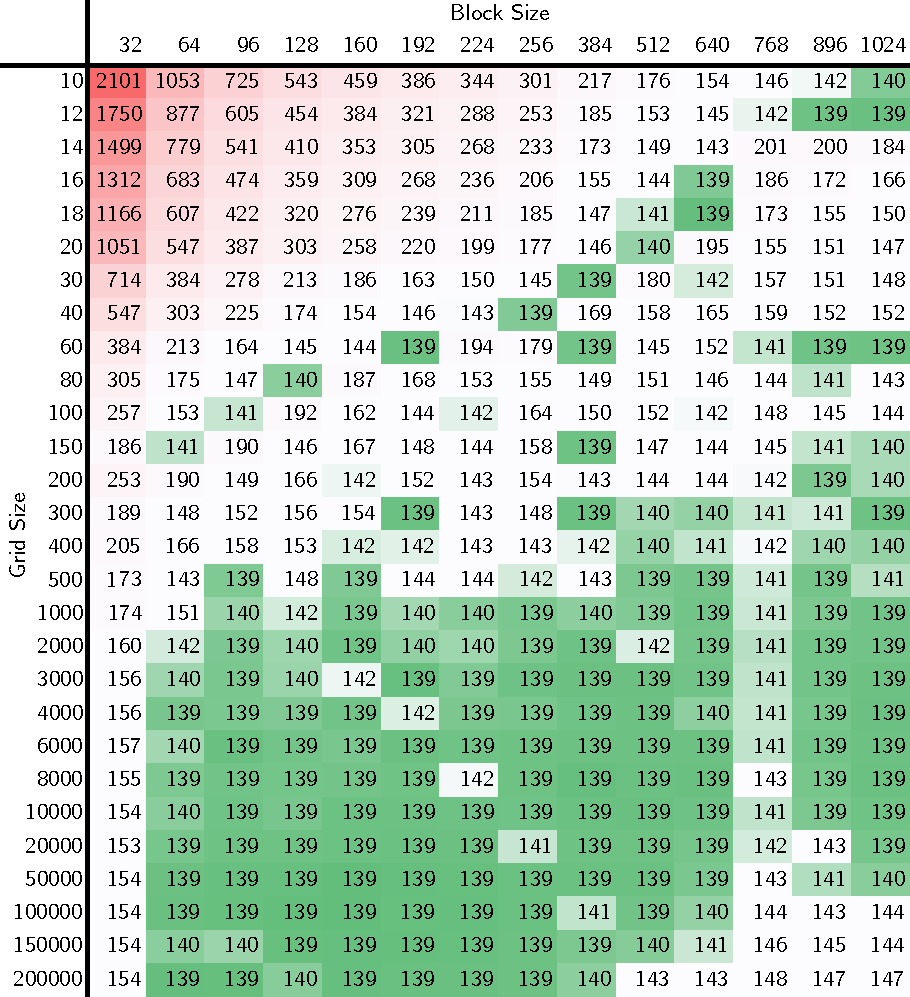
\includegraphics[]{bilder/parameter64.pdf}
	\caption{Laufzeit des String-Vergleichsalgorithmus in ms für den Type-Datensatz mit einer Selektivität von 64\% unter Verwendung unterschiedlicher Grid-Konfigurationen}
\end{figure}